\documentclass[a4paper]{article}
\usepackage[english]{babel}
\usepackage[utf8]{inputenc}
\usepackage{textcomp}
\usepackage{amsmath}
\usepackage{gensymb}
\usepackage{physics}
\usepackage{graphicx}
\usepackage[colorinlistoftodos]{todonotes}
\usepackage{xcolor}
\usepackage{array}
\usepackage{tabularx}
\usepackage{tikz}
\usepackage{pgfplots}
\usepackage{framed}
\usepackage{xfrac}
\usepackage[most]{tcolorbox}
\usepackage{fix-cm}
\usepackage[margin=0.5in]{geometry}
\usetikzlibrary{quotes,angles}
\usetikzlibrary{decorations.pathreplacing}
\usetikzlibrary{calc}
\usepgfplotslibrary{fillbetween}

\let\phi\varphi
\let\bf\textbf
\colorlet{shadecolor}{orange!15}
\pgfplotsset{compat=1.18}
\newcommand\der[2]{\frac{d #1}{d #2}}
\newcommand\Deltat{\Delta t}
\newcommand\rads{\text{ rad\;s}^{-1}}
\newcommand\radss{\text{ rad\;s}^{-2}}
\newcommand\rad{\text{ rad}}
\newcommand\s{\text{ s}}
\newcommand\ms{\text{ ms}^{-1}}
\newcommand\mss{\text{ ms}^{-2}}
\newcommand\kgms{\text{kg\;ms}^{-1}}
\def\centerarc[#1](#2)(#3:#4:#5){\draw[#1] ($(#2)+({#5*cos(#3)},{#5*sin(#3)})$) arc (#3:#4:#5)}
% Syntax: \centerarc[draw options] (center) (initial angle:final angle:radius);

\title{Fixed-Axis Rotation}
\author{OpenStax University Physics Vol. 1}
\date{}

\begin{document}
\setcounter{section}{10}
\maketitle
\subsection{Rotational Variables}
\noindent\bf{Angular Velocity}
\vspace{2mm}\\
Uniform circular motion is motion in a circle at constant speed, although this is the simplest case of rotational motion, it is used here to introduce rotational variables.\par
The figure shows a particle moving in a circle. Its position vector from the origin of the circle to the particle sweeps out the angle $\theta$, which increases in the counterclockwise direction as the particle moves along its path. The angle $\theta$ is called the angular position of the particle. As the particle moves, it traces an arc length $s$.
\begin{center}
    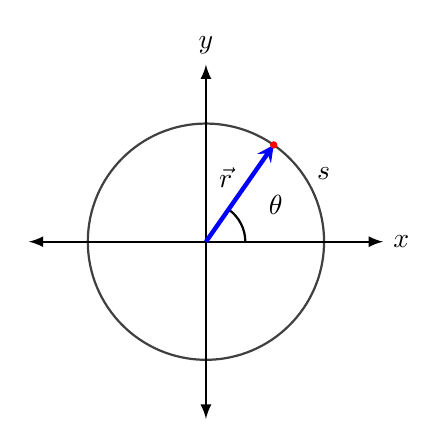
\begin{tikzpicture}[scale=1.5]
        %%% COORDINATES %%%
        \draw (0,0) coordinate (o);
        \draw ({cos(55)},{sin(55)}) coordinate (a);
        \draw ({cos(55)},0) coordinate (b);

        %%% AXES & CIRCLE %%%
        \draw[thick,draw=black!75] (0,0) circle (1);
        \draw[<->,thick,-latex] (0,0)--(1.5,0) node[right]{$x$};
        \draw[<->,thick,-latex] (0,0)--(0,1.5) node[above]{$y$};
        \draw[<->,thick,-latex] (0,0)--(-1.5,0);
        \draw[<->,thick,-latex] (0,0)--(0,-1.5);

        %%% POSITION VECTOR & ANGLE %%%
        \draw pic["$\theta$",draw=black,thick,-,angle eccentricity=2,angle radius=0.5cm]{angle=b--o--a};
        \draw[->,ultra thick,draw=blue,-stealth] (0,0)--node[left,xshift=0.5mm,yshift=2mm]{$\vec{r}$}({cos(55)},{sin(55)});

        \centerarc[red,very thick](0,0)(0:55:1);
        \node at ({1.15*cos(30)},{1.15*sin(30)}){$s$};
        \filldraw[red] ({cos(55)},{sin(55)}) circle (0.75pt);
    \end{tikzpicture}
\end{center}
The angle is related to the radius of the circle and the arc length by 
\begin{equation}
    \theta = \frac{s}{r}
\end{equation}
The angle $\theta$, the angular position of the particle moving along its path has units of radians (rad). As the particle moves along its circular path, its angular position changes and it undergoes angular displacements $\Delta\theta$.\par\vspace{1mm}
\noindent We can assign vectors to the quantities in equation 1, the angle $\vec{\theta}$ is a vector out of the page. The angular position vector $\vec{r}$ and the arc length vector $\vec{s}$ both lie in the plane of the page, they are related by:
\begin{equation}
    \vec{s} = \vec{\theta} \times \vec{r}
\end{equation}
The arc length is the cross product of the angle vector and the position vector
\begin{center}
    \begin{tikzpicture}[scale=2]
        \draw[->,-latex] (0,0)--(1,0) node[right]{$y$};
        \draw[->,-latex] (0,0)--(0,1) node[above]{$z$};
        \draw[->,-latex] (0,0)--(-{cos(45)},-{sin(45)}) node[left]{$x$};

        \draw[->,very thick,-stealth] (0,0)--node[right]{$\vec{\theta}$}(0,0.75);
        \draw[->,very thick,-stealth] (0,0)--node[below,xshift=-2mm,yshift=0.5mm]{$\vec{r}$}({0.7*cos(65)},{-0.7*cos(65)});
        \draw[->,very thick,-stealth,draw=red] ({0.7*cos(65)},{-0.7*cos(65)})--node[right,yshift=-1mm,xshift=-0.5mm]{$\vec{s}$}({0.7*cos(65) + 0.28},{-0.7*cos(65) + 0.28});
    \end{tikzpicture}
\end{center}
The magnitude of the angular velocity, denoted by $\omega$, is the time rate of change of the angle $\theta$ as the particle moves in a circular path. The instantaneous angular velocity, defined as the limit as $\Delta t \to 0$ of the average angular velocity $\bar{\omega} = \frac{\Delta\theta}{\Delta t}$
\begin{equation}
    \omega = \lim\limits_{\Delta t \to 0}\frac{\Delta\theta}{\Delta t} = \frac{d\theta}{dt}
\end{equation}
Where $\theta$ is the angle of rotation. The units of angular velocity are radians per second (rad\;s$^{-1}$). Angular velocity can also be referred to as the rotation rate in radians per second. In many cases, rotation rate is given in revolutions/s or cycles/s, to find angular velocity, multiply revolutions/s by $2\pi$ (since there are $2\pi$ radians per revolution). Since a positive angle in a circle is counterclockwise, we take counterclockwise rotations as being positive and clockwise rotations as negative.\vspace{1mm}\par
\noindent We can see how angular velocity is related to the tangential speed of the particle by differentiating equation 1 with respect to time. Equation 1 can be rewritten as:
\begin{align*}
    s = \theta r
\end{align*}
\newpage
\noindent Taking the derivative with respect to time and noting that the radius $r$ is constant gives:
\begin{align*}
    \der{s}{t} = \der{}{t}(r\theta) = \theta\der{r}{t} + r\der{\theta}{t} = r\der{\theta}{t}
\end{align*}
Where $\theta\der{r}{t} = 0$. Here, $\der{s}{t}$ is just the tangential speed $v_t$ of the particle moving in a circular path. Using equation 3 we arrive at:
\begin{equation}
    v_t = r\omega
\end{equation}
The tangential speed of the particle is its angular velocity times the radius of the circle. The tangential speed of the particle increases with its distance from the axis of rotation for a constant angular velocity. The figure shows two particles placed at different radii on a rotating disk with constant angular velocity. As it rotates, the tangential speed increases linearly with the radius from the axis of rotation. We see that $v_1 = r_1\omega_1$ and $v_2 = r_2\omega_2$. The disk has a constant angular velocity so $\omega_1 = \omega_2$. This means that $\frac{v_1}{r_1} = \frac{v_2}{r_2}$ or $v_2 = \big(\frac{r_2}{r_1}\big)$. Thus, since $r_2 > r_1$, $v_2 > v_1$
\begin{center}
    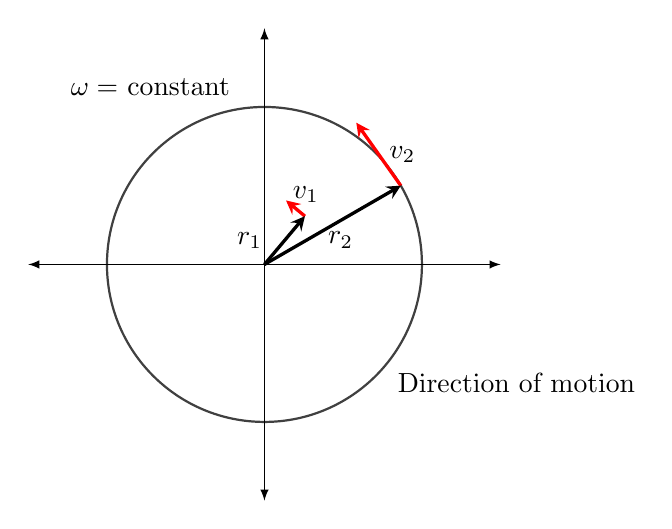
\begin{tikzpicture}[scale=2]
        %%% COORDINATES %%%
        \draw (0,0) coordinate (O);
        \draw ({cos(30)},{sin(30)}) coordinate (a);
        \draw ({0.4*cos(50)},{0.4*sin(50)}) coordinate (b);

        %%% AXES & CIRCLE %%%
        \draw[thick,draw=black!75] (0,0) circle (1);
        \draw[->,-latex] (O)--(1.5,0);
        \draw[->,-latex] (O)--(-1.5,0);
        \draw[->,-latex] (O)--(0,1.5);
        \draw[->,-latex] (O)--(0,-1.5);

        %%% LINES %%%
        \draw[->,very thick,-stealth,draw=red] (a)--node[right]{$v_2$}({cos(30) - 0.4*cos(45)},{sin(30) + 0.4});
        \draw[->,very thick,-stealth,draw=red] (b)--({0.4*cos(50) - 0.17*cos(45)},{0.4*sin(50) + 0.1}) node[right,yshift=0.75mm,xshift=-0.5mm]{$v_1$};
        \draw[->,very thick,-stealth] (O)--node[below,xshift=1mm,yshift=0.5mm]{$r_2$}(a);
        \draw[->,very thick,-stealth] (O)--node[left,xshift=-1.5mm]{$r_1$}(b);

        \node at ({-1.45*cos(60)},{1.3*sin(60)}){$\omega =$ constant};

        \centerarc[->,black!50,thick,-stealth](0,0)(-30:-10:1.1);
        \centerarc[->,black!50,thick,-stealth](0,0)(60:80:1.1);
        \centerarc[->,black!50,thick,-stealth](0,0)(150:170:1.1);
        \centerarc[->,black!50,thick,-stealth](0,0)(240:260:1.1);
        \node at (1.6,-0.75){Direction of motion};
    \end{tikzpicture}
\end{center}
Similar to equation 2, one can state a cross product relation to the vector of the tangential velocity as stated in equation 4, therefore:
\begin{equation}
    \vec{v} = \vec{\omega} \times \vec{r}
\end{equation}
The tangential velocity is the cross product of the angular velocity and the position vector as shown below. On the left we see that with the angular velocity in the $+z$ direction, the rotation in the $xy$ plane is counterclockwise. On the right, the angular velocity is in the $-z$ direction, which gives a clockwise rotation in the $xy$ plane.
\begin{center}
    \begin{tikzpicture}[scale=2]
        \draw[->,-latex] (0,0)--(1,0) node[right]{$y$};
        \draw[->,-latex] (0,0)--(0,1) node[above]{$z$};
        \draw[->,-latex] (0,0)--(-{cos(45)},-{sin(45)}) node[left]{$x$};

        \draw[->,very thick,-stealth] (0,0)--node[right]{$\vec{\omega}$}(0,0.75);
        \draw[->,very thick,-stealth,draw=red] ({0.7*cos(65)},{-0.7*cos(65)})--node[right,yshift=-1mm,xshift=-0.5mm]{$\vec{v}$}({0.7*cos(65) + 0.26},{-0.7*cos(65) + 0.26});
        \draw[->,very thick,-stealth] (0,0)--node[below,xshift=-2mm,yshift=0.5mm]{$\vec{r}$}({0.7*cos(65)},{-0.7*cos(65)});
    \end{tikzpicture}
    \hspace{15mm}
    \begin{tikzpicture}[scale=2]
        \draw[->,-latex] (0,0)--(1,0) node[right]{$y$};
        \draw[->,-latex] (0,0)--(0,1) node[above]{$z$};
        \draw[->,-latex] (0,0)--(-{cos(45)},-{sin(45)}) node[left]{$x$};

        \draw[->,very thick,-stealth] (0,0)--node[left]{$\vec{\omega}$}(0,-0.75);
        \draw[->,very thick,-stealth,draw=red] ({0.7*cos(65)},{-0.7*cos(65)})--node[right,yshift=-1mm,xshift=-0.5mm]{$\vec{v}$}({0.7*cos(65) - 0.26},{-0.7*cos(65) - 0.26});
        \draw[->,very thick,-stealth] (0,0)--node[above,yshift=-1.5mm,xshift=1.5mm]{$\vec{r}$}({0.7*cos(65)},{-0.7*cos(65)});
    \end{tikzpicture}
\end{center}
\begin{shaded}
    \underline{\bf{Example 10.1:} Rotation of a Flywheel}
    \vspace{2mm}\\
    A flywheel rotates such that it sweeps out an angle at the rate of $\theta = \omega t = (45.0\text{ rad\;s}^{-1})t$ radians. The wheel rotates counterclockwise when viewed in the plane of the page.
    \begin{enumerate}
        \item[(a)] What is the angular velocity $\omega$ of the flywheel?
        \vspace{1mm}\\
        $\displaystyle \omega = \der{\theta}{t} = 45$ rad\;s$^{-1}$, angular velocity is constant
        \item[(b)] What direction is the angular velocity?
        \vspace{1mm}\\
        The direction of rotation is counterclockwise, so the direction of angular velocity is $+z$
        \item[(c)] How many radians does the flywheel rotate through in 30 s?
        \vspace{1mm}\\
        $\displaystyle \theta(t) = \omega t \to \Delta\theta = \theta(30$ s$) - \theta(0$ s$) = \theta(30$ s$) \to (45.0$ rad\;s$^{-1})(30$ s$) = 1350.0$ rad
        \item[(d)] What is the tangential speed of a point on the flywheel 10 cm from the axis of rotation
        \vspace{1mm}\\
        $v_t = r\omega = (0.1$ m$)(45.0$ rad\;s$^{-1}) = 4.5$ ms$^{-1}$
    \end{enumerate}
\end{shaded}
\newpage
\noindent\bf{Angular Acceleration}
\vspace{2mm}\\
For describing situations where $\omega$ changes, we need to define angular acceleration. The faster the change in $\omega$, the greater the angular acceleration. Instantaneous angular acceleration $\alpha$ is defined as the derivative of angular velocity with respect to time:
\begin{equation}
    \alpha = \lim_{\Delta t \to 0}\frac{\Delta\omega}{\Delta t} = \der{\omega}{t} = \frac{d^2\theta}{dt^2}
\end{equation}
Where we have taken the limit of the average angular acceleration $\bar{\alpha} = \frac{\Delta\omega}{\Delta t}$ as $\Delta t \to 0$. The units of angular acceleration are radians/s per second, or rad\;s$^{-2}$. 
\vspace{1mm}\par
\noindent In the same way that the vector associated with angular velocity $\vec{\omega}$ was defined, we can define $\vec{\alpha}$, the vector associated with angular acceleration. If the angular velocity is along the $+z$ axis and $\der{\omega}{t}$ is positive, the angular acceleration $\vec{\alpha}$ is positive and points along the $+z$ axis, if $\der{\omega}{t}$ is negative, the angular acceleration is negative and points along the $-z$ axis.

\begin{center}
    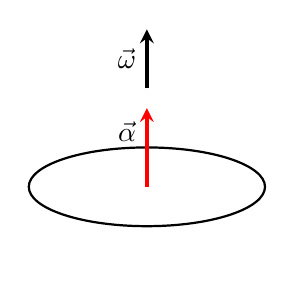
\begin{tikzpicture}
        \draw[thick] (0,0) ellipse (1.5 and 0.5);
        \draw (0,0) coordinate (O);
        \draw[->,very thick,-stealth,draw=red] (O)--node[left,yshift=2mm]{$\vec{\alpha}$}(0,1);
        \draw[->,very thick,-stealth] (0,1.25)--node[left]{$\vec{\omega}$}(0,2);
        \centerarc[->,black!50,thick,-stealth](0,0)(-10:10:1.7);
        \node at (0,-1){};
    \end{tikzpicture}
    \hspace{15mm}
    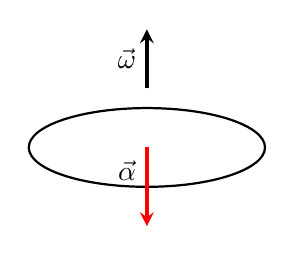
\begin{tikzpicture}
        \draw[thick] (0,0) ellipse (1.5 and 0.5);
        \draw (0,0) coordinate (O);
        \draw[->,very thick,-stealth,draw=red] (O)--node[left,yshift=2mm]{$\vec{\alpha}$}(0,-1);
        \draw[->,very thick,-stealth] (0,0.75)--node[left]{$\vec{\omega}$}(0,1.5);
        \centerarc[->,black!50,thick,-stealth](0,0)(-10:10:1.7);
    \end{tikzpicture}
\end{center}
The tangential acceleration vector can be expressed as a cross product of the angular acceleration and position vectors. This equation can be found by taking the derivative of equation 5
\begin{equation}
    \vec{a} = \vec{\alpha} \times \vec{r}
\end{equation}
The vector relationships for angular acceleration and tangential acceleration are shown below
\begin{center}
    \begin{tikzpicture}[scale=2]
        \draw[->,-latex] (0,0)--(1,0) node[right]{$y$};
        \draw[->,-latex] (0,0)--(0,1) node[above]{$z$};
        \draw[->,-latex] (0,0)--(-{cos(45)},-{sin(45)}) node[left]{$x$};

        \draw[->,very thick,-stealth] (0,0)--node[right]{$\vec{\alpha}$}(0,0.75);
        \draw[->,very thick,-stealth,draw=red] ({0.7*cos(65)},{-0.7*cos(65)})--node[right,yshift=-1mm,xshift=-0.5mm]{$\vec{a}$}({0.7*cos(65) + 0.26},{-0.7*cos(65) + 0.26});
        \draw[->,very thick,-stealth] (0,0)--node[below,xshift=-2mm,yshift=0.5mm]{$\vec{r}$}({0.7*cos(65)},{-0.7*cos(65)});
    \end{tikzpicture}
    \hspace{15mm}
    \begin{tikzpicture}[scale=2]
        \draw[->,-latex] (0,0)--(1,0) node[right]{$y$};
        \draw[->,-latex] (0,0)--(0,1) node[above]{$z$};
        \draw[->,-latex] (0,0)--(-{cos(45)},-{sin(45)}) node[left]{$x$};

        \draw[->,very thick,-stealth] (0,0)--node[left]{$\vec{\alpha}$}(0,-0.75);
        \draw[->,very thick,-stealth,draw=red] ({0.7*cos(65)},{-0.7*cos(65)})--node[right,yshift=-1mm,xshift=-0.5mm]{$\vec{a}$}({0.7*cos(65) - 0.26},{-0.7*cos(65) - 0.26});
        \draw[->,very thick,-stealth] (0,0)--node[above,yshift=-1.5mm,xshift=1.5mm]{$\vec{r}$}({0.7*cos(65)},{-0.7*cos(65)});
    \end{tikzpicture}
\end{center}
Tangential acceleration of a point on a rotating body at a distance from the axis of rotation can be related in the same way as tangential velocity and angular velocity. Differentiating equation 4 with respect to time (the radius $r$ is constant) gives:
\begin{equation}
    a_t = r\alpha
\end{equation}
The tangential acceleration $a_t$ is the radius times the angular acceleration
\begin{shaded}
    \underline{\bf{Example 10.2:} A Spinning Bike Wheel}
    \vspace{2mm}\\
    A bicycle mechanic mounts a bicycle on the repair stand and starts the rear wheel spinning from rest to a final angular velocity of 250 rpm in 5.00 s.
    \begin{enumerate}
        \item[(a)] Calculate the average angular acceleration in rad\;s$^{-2}$
        \begin{align*}
            \displaystyle \bar{\alpha} = \frac{\Delta\omega}{\Delta t} = \frac{250\text{ rpm}}{5.00\text{ s}}
        \end{align*}
        Converting from rpm to rad\;s$^{-1}$:
        \begin{align*}
            \Delta\omega = 250\frac{\text{rev}}{\text{min}} \cdot \frac{2\pi\text{ rad}}{\text{rev}} \cdot \frac{1\text{ min}}{60\text{ s}} = 26.2\text{rad\;s}^{-1}
        \end{align*}
        Entering this back into the expression for $\alpha$ gives:
        \begin{align*}
            \alpha = \frac{\Delta\omega}{\Delta t} = \frac{26.2\text{ rad\;s}^{-1}}{5.00\text{ s}} = 5.24\text{ rad\;s}^{-2}
        \end{align*}
        \item[(b)] If the brakes are hit, causing an angular acceleration of -87 rad\;s$^{-2}$, how long does it take the wheel to stop?
        \vspace{1mm}\\
        Angular velocity decreases from 26.2 rad\;s$^{-1}$ to zero so $\Delta\omega = -26.2$ rad\;s$^{-1}$, and $\alpha$ is given to be -87.3 rad\;s$^{-2}$
        \begin{align*}
            \Delta t = \frac{\Delta\omega}{\alpha} = \frac{-26.2\text{ rad\;s}^{-1}}{-87.3\text{ rad\;s}^{-2}} = 0.300\text{ s}
        \end{align*}
    \end{enumerate}
\end{shaded}

\newpage
\begin{shaded}
    \underline{\bf{Example 10.3:} Wind Turbine}
    \vspace{2mm}\\
    A wind turbine in a wind farm is being shut down for maintenance. It takes 30 s for the turbine to go from its operating angular velocity to a complete stop in which the angular velocity function is $\omega(t) = \Big[\frac{(t\text{s}^{-1} - 30.0)^2}{100.0}\Big]$rad\;s$^{-1}$, where $t$ is the time in seconds. If the turbine is rotating counterclockwise looking into the page:
    \begin{enumerate}
        \item[(a)] What are the directions of the angular velocity and acceleration vectors?
        \vspace{1mm}\\
        Since the turbine is rotating counterclockwise, angular velocity $\vec{\omega}$ points towards $+z$. Since the angular velocity is decreasing, the angular acceleration $\vec{\alpha}$ points towards $-z$
        \item[(b)] What is the average angular acceleration?
        \vspace{1mm}\\
        At $t = 0$, the initial angular velocity of the turbine is $\omega = 9.0$ rad\;s$^{-1}$, the final angular velocity is zero, so the average angular velocity $\bar{\alpha}$ is:
        \begin{align*}
            \bar{\alpha} = \frac{\Delta\omega}{\Delta t} = \frac{\omega - \omega_0}{t - t_0} = \frac{0 - 9.0\text{ rad\;s}^{-1}}{30.0 - 0\text{ s}} = -0.3\text{ rad\;s}^{-2}
        \end{align*}
        \item[(c)] What is the instantaneous angular acceleration at $t = 0.0, 15.0, 30.0$ s?
        \vspace{1mm}\\
        Taking the derivative of angular velocity with respect to time gives
        \begin{align*}
            \alpha = \der{\omega}{t} = \bigg[\frac{(t - 30.0)}{50.0}\bigg]\text{ rad\;s}^{-2}
        \end{align*}
        Thus:\hspace{2.5mm} $\alpha(0.0\text{ s}) = -0.6$ rad\;s$^{-2}$, $\alpha(15.0\text{ s}) = -0.3$ rad\;s$^{-2}$, and $\alpha(30.0\text{s}) = 0$ rad\;s$^{-2}$
    \end{enumerate}
\end{shaded}

\newpage
\subsection{Rotation With Constant Angular Acceleration}
In this section, the definitions from the previous section are used to derive relationships among these variables, and use these relationships to analyze rotational motion for a rigid body about a fixed axis under a constant angular acceleration, forming the basis for rotational kinematics. If angular acceleration is constant, the equations of rotational kinematics simplify, similar to the equations of linear kinematics. 
\vspace{2mm}\\
\bf{Kinematics of Rotational Motion}
\vspace{2mm}\\
In the previous section we saw that if a flywheel has an angular acceleration in the same direction as its angular velocity, its angular velocity increases with time and its angular displacement also increases. If the angular acceleration is opposite to the angular velocity vector, its angular velocity decreases with time. Under a constant angular acceleration, we can describe these physical situations with a consistent set of rotational kinematic equations.
\vspace{2mm}\\
If the system is rotating under a constant acceleration, then the average angular velocity follows a simple relation because the angular velocity is increasing linearly with time. The average angular velocity is just half of the sum of the initial and final values:
\begin{equation}
    \bar{\omega} = \frac{\omega_0 + \omega_f}{2}
\end{equation}
Using the definition of average angular velocity, an equation that relates the angular position, average angular velocity, and time can be found:
\begin{align*}
    \bar{\omega} = \frac{\Delta\theta}{\Delta t}
\end{align*}
Solving for $\theta$ gives:
\begin{equation}
    \theta_f = \theta_0 + \bar{\omega}t
\end{equation}
Where $t_0 = 0$. This equation can be useful when the average angular velocity of the system is known. Then the angular displacement over a given period of time could be found. To determine an equation relating $\omega, \alpha$, and $t$, we start with the definition of angular acceleration:
\begin{align*}
    \alpha = \der{\omega}{t}
\end{align*}
This is rearranged to $\alpha dt = d\omega$, then we integrate both sides of the equation from initial to final values, from $t_0$ to $t$ and from $\omega_0$ to $\omega_f$. (angular acceleration is constant and can be pulled outside)
\begin{align*}
    \alpha\int_{t_0}^{t}dt = \int_{\omega_0}^{\omega_f}d\omega
\end{align*}
Setting $t_0 = 0$ gives:
\begin{align*}
    \alpha t = \omega_f - \omega_0
\end{align*}
This is rearranged to obtain 
\begin{equation}
    \omega_f = \omega_0 + \alpha t
\end{equation}
Where $\omega_0$ is the initial angular velocity. This equation is the rotational counterpart to the linear kinematic equation $v_f = v_0 + at$. With equation 11, the angular velocity of an object at any specified time $t$ can be found given the initial angular velocity and angular acceleration.
\vspace{1mm}\\
Doing a similar thing to the equation $\omega = \der{\theta}{t}$, rearranging it to $\omega dt = d\theta$ and integrating both sides from initial to final values, noting that angular acceleration is constant and does not have a time dependence. This time angular velocity is not constant, so equation 11 is substituted in:
\begin{align*}
    \int_{t_0}^{t_f}(\omega_0 + \alpha t)dt &= \int_{\theta+0}^{\theta_f}d\theta\\
    \int_{t_0}^{t}\omega_0dt + \int_{t_0}^{t}\alpha t dt &= \int_{\theta_0}^{\theta_f}d\theta\\
    \bigg[\omega_0t + \frac{1}{2}\alpha t^2\bigg]_{t_0}^t = \omega_0t + &\frac{1}{2}\alpha t^2 = \theta_f - \theta_0
\end{align*}
Where $t_0 = 0$. Now we rearrange to obtain:
\begin{equation}
    \theta_f = \theta_0 + \omega_0t + \frac{1}{2}\alpha t^2
\end{equation}
This is the rotational counterpart to the linear kinematic equation $s_f = s_0 + v_0t + \frac{1}{2}at^2$. This equation gives the angular position of a rotating rigid body at any time $t$ given the initial conditions ($\theta_0$ and $\omega_0$) and the angular acceleration
\newpage
\noindent We can find an equation that is independent of time by solving for $t$ in equation 11 and substituting into equation 12:
\begin{align*}
    \theta_f &= \theta_0 + \omega_0 \bigg(\frac{\omega_f - \omega_0}{\alpha}\bigg) + \frac{1}{2}\alpha \bigg(\frac{\omega_f - \omega_0}{\alpha}\bigg)^2\\
    &= \theta_0 + \frac{\omega_0\omega_f}{\alpha} - \frac{\omega_0^2}{\alpha} + \frac{1}{2}\frac{\omega_f^2}{\alpha} - \frac{\omega_0\omega_f}{\alpha} + \frac{1}{2}\frac{\omega_0^2}{\alpha}\\
    &= \theta_0 + \frac{1}{2}\frac{\omega_f^2}{\alpha} - \frac{1}{2}\frac{\omega_0^2}{\alpha}\\
    \theta_f - \theta_0 &= \frac{\omega_f^2 - \omega_0^2}{2\alpha}
\end{align*}
This rearranges to:
\begin{equation}
    \omega_f^2 = \omega_0^2 + 2\alpha(\Delta\theta)
\end{equation}
Equations 10 - 13 describe fixed-axis rotation for constant acceleration and are summarized below
\begin{center}
    \begin{tabularx}{0.4\textwidth}{ 
        | >{\raggedright\arraybackslash}X  
        | >{\raggedright\arraybackslash}X |}
        \hline
        Rotational & Linear\\[2.5pt]
        \hline
        $\theta_f = \theta_0 + \bar{\omega}t$ & $s_f = s_0 + \bar{v}t$\\[2.5pt]
        \hline
        $\omega_f = \omega_0 + \alpha t$ & $v_f = v_0 + at$\\[2.5pt]
        \hline
        $\theta_f = \theta_0 + \omega_0t + \frac{1}{2}\alpha t^2$ & $s_f = s_0 + v_0t + \frac{1}{2}at^2$\\[2.5pt]
        \hline
        $\omega_f^2 = \omega_0^2 + 2\alpha(\Delta\theta)$ & $v_f^2 = v_0^2 + 2a(\Delta s)$\\[2.5pt]
        \hline
    \end{tabularx}
\end{center}

\begin{shaded}
    \underline{\bf{Example: 10.4/5} Calculating the Acceleration of a Fishing Pole}
    \vspace{2mm}\\
    A deep-sea fisherman hooks a big fish that swims away from the boat, pulling the fishing line from his fishing reel. The whole system is initially at rest, and the fishing line unwinds from the reel at a radius of 4.50 cm from its axis of rotation. The reel is given an angular acceleration of 110 rad\;s$^{-2}$ for 2.00 s
    \begin{enumerate}
        \item[(a)] What is the final velocity of the reel after 2 s?
        \vspace{1mm}\\
        Since $\alpha$ and $t$ are given, the most straightforward equation to use to find $\omega$ is $\omega_f = \omega_0 + \alpha t$. Because the system starts from rest, $\omega_0 = 0$, so:
        \begin{align*}
            \omega_f = 0 + (110\text{ rad\;s}^{-2})(2.00\text{ s}) = 220\text{ rad\;s}^{-1}
        \end{align*}
        \item[(b)] How many revolutions does the reel make? 
        \vspace{1mm}\\
        To find the number of revolutions, find $\theta$ in radians (1 rev = $2\pi$ rad). $\alpha$ and $t$ are given, and $\omega_0 = 0$, so $\theta$ can be obtained by using:
        \begin{align*}
            \theta_f &= \theta_0 + \omega_0t + \frac{1}{2}\alpha t^2\\
            &= 0 + 0 + \frac{1}{2}\Big(110\text{ rad\;s}^{-2}\Big)(2.00\text{ s})^2\\
            &= 200\text{ rad}
        \end{align*}
        Converting from radians to revolutions:
        \begin{align*}
            (220\text{ rad})\bigg(\frac{1\text{ rev}}{2\pi\text{ rad}}\bigg) = 35.0\text{ rad}
        \end{align*}
        \item[(c)] Now the fisherman applies a brake to the spinning wheel, achieving an angular acceleration of -300 rad\;s$^{-2}$. How long does it take for the reel to come to a stop?
        \vspace{1mm}\\
        Solving the equation $\omega_f = \omega_0 + \alpha t$ for $t$, and substituting in known values gives:
        \begin{align*}
            t = \frac{\omega_f - \omega_0}{\alpha} = \frac{0 - 220.0\text{ rad\;s}^{-1}}{-300\text{ rad\;s}^{-2}} = 0.733\text{ s}
        \end{align*}
    \end{enumerate}
\end{shaded}

\newpage
\begin{shaded}
    \underline{\bf{Example 10.6:} Angular Acceleration of a Propeller}
    \vspace{2mm}\\
    The figure shows a graph of the angular velocity of a propeller on an aircraft as a function of time. Its angular velocity starts at 30$\rads$ and drops linearly to 0$\rads$ over the course of 5 s.
    \begin{center}
        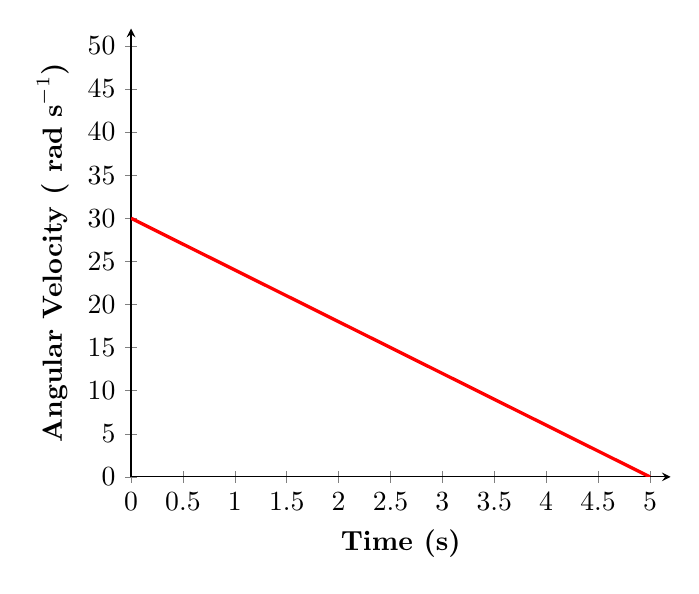
\begin{tikzpicture}
            \begin{axis}[
                axis lines=left,
                xlabel=\bf{Time (s)},
                ylabel=\bf{Angular Velocity ($\rads$)},
                xmax=5.2,
                ymax=52,
                xtick distance=0.5,
                ytick distance=5,
            ]
            \addplot[
                very thick,
                domain=0:5,
                samples=100,
                color=red,
                name path=A,
            ]
            {-6*x + 30};
                
            \end{axis}
        \end{tikzpicture}
    \end{center}
    \begin{enumerate}
        \item[(a)] Find the angular acceleration of the object and verify the result using kinematic equations
        \vspace{1mm}\\
        Because angular velocity varies linearly with time, angular acceleration is constant and not dependent on time. The angular acceleration is the derivative of angular velocity, $\alpha = \der{\omega}{t}$. At $t = 0$ s, $\omega_0 = 30\rads$ and at $t = 5$ s, $\omega_f = 0\rads$
        \begin{align*}
            \alpha = \frac{\omega - \omega_0}{t - t_0} = \frac{(0 - 30.0)\rads}{(5.0 - 0)\s} = -6.0\radss
        \end{align*}
        \item[(b)] Find the angle through which the propeller rotates during these 5 seconds and verify your result using kinematic equations
        \vspace{1mm}\\
        Since $\omega = \der{\theta}{t}$, angular displacement $\Delta\theta$ can be calculated by integrating the angular velocity
        \begin{align*}
            \int_{\theta_0}^{\theta_f}d\theta = \theta_f - \theta_0 = \int_{t_0}^{t_f}\omega(t)dt
        \end{align*}
        The area under the curve can be found by calculating the area of the right triangle shown:
        \begin{center}
            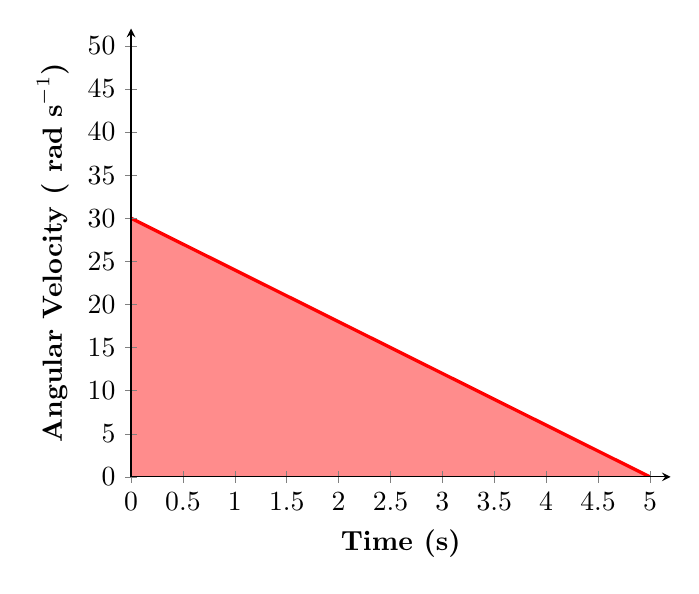
\begin{tikzpicture}
                \begin{axis}[
                    axis lines=left,
                    xlabel=\bf{Time (s)},
                    ylabel=\bf{Angular Velocity ($\rads$)},
                    xmax=5.2,
                    ymax=52,
                    xtick distance=0.5,
                    ytick distance=5,
                    axis on top,
                ]
                \addplot[
                    very thick,
                    domain=0:5,
                    samples=100,
                    color=red,
                    name path=A,
                ]
                {-6*x + 30};
                \path[name path=B]
                    (axis cs:\pgfkeysvalueof{/pgfplots/xmin},0)--
                    (axis cs:\pgfkeysvalueof{/pgfplots/xmax},0);
                \addplot[red!45] fill between[of=A and B,soft clip={domain=0:5},];
                \end{axis}
            \end{tikzpicture}
        \end{center}
        \begin{align*}
            \Delta\theta &= A(\text{triangle}) = \frac{1}{2}l \times h\\
            \Delta\theta &= \frac{1}{2}\Big(30\rads\Big)(5\s)
        \end{align*}
        This is verified using equation 12 ($\theta_f = \theta_0 + \omega_0t + \frac{1}{2}\alpha t^2$), and setting $\theta_0 = 0$ gives:
        \begin{align*}
            \theta_f = \big(30.0\rads\big)(5.0\s) + \frac{1}{2}\big(-6.0\radss\big)\big(5.0\rads\big)^2 = 150.0 - 75.0 = 75.0\rad
        \end{align*}
    \end{enumerate}
\end{shaded}

\end{document}